\subsection{Kubernetes}
\label{s:ProblemDomain:Kubernetes}

One of the most advanced and popular container management tools available today is \emph{Kubernetes}, a platform for container orchestration, often used in a vast range of projects with virtualized work environments.
It is a next-generation successor \cite{b:Borg-K8s-predecessor} to the Borg cluster manager.
Within its responsibilities lies e.g., resource allocation, container monitoring, and handling failovers.
Being an open-source solution, it is also extensible \cite{b:Kubernetes-what-is}, which enables the user to integrate their own custom extensions over a predefined interface to adjust core functionalities to their needs. A top level architecture of Kubernetes cluster is presented in \cref{fig:kubernetes:architecture} and consists of a control plane that serves a role akin to the cluster's master node and worker nodes.

%%%%
\begin{figure}[H]
\centering
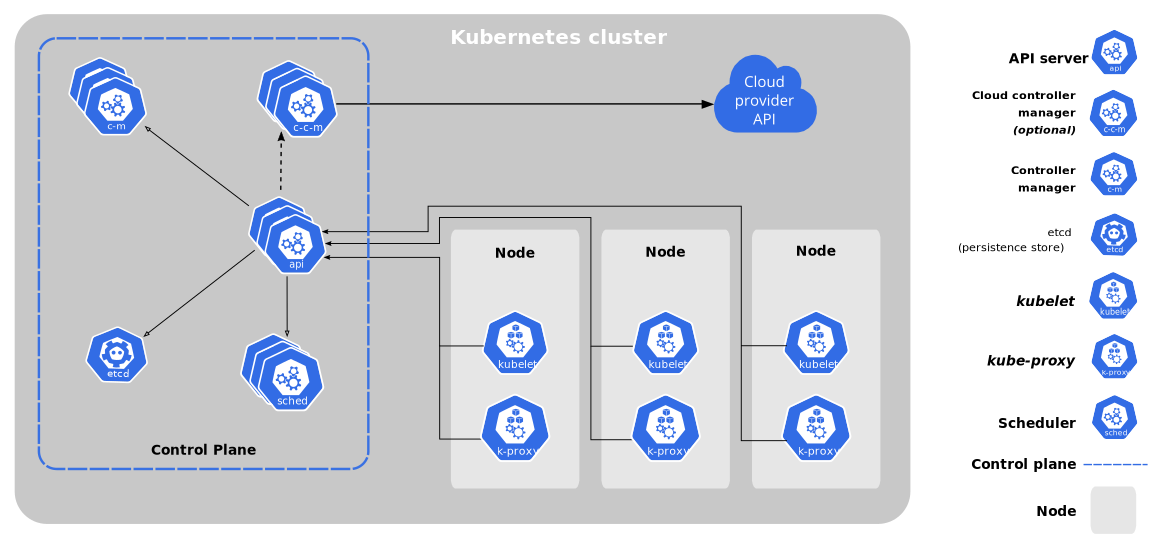
\includegraphics[width=1\linewidth]{figures/2-1-k8s-arch.png}
\caption[Kubernetes cluster architecture diagram]{A diagram\footnotemark of Kubernetes cluster components and processes distributed among them.}

% \medskip
% \begin{minipage}{0.65\textwidth}
% {\footnotesize Depicts Kubernetescluster components and processes distributed among them.\par}
% \end{minipage}

\label{fig:kubernetes:architecture}
\end{figure}
\footnotetext{Source: \url{https://kubernetes.io/docs/concepts/overview/components}, Access: 2021-05-26}
%%%%

With an exposed \emph{Application Programmable Interface (API)} workloads can be dynamically scheduled by any authorized third-party application.
They are represented in a form of a configuration file called \emph{deployment}, which contains details of the requested Kubernetes resources such as pods or services.

%%%%%%%



\subsubsection{Pod}\label{s:ProblemDomain:Kubernetes:pod}

A base workload type in Kubernetes is called \emph{pod} and is meant to represent a standalone working process. 
It is used as an abstraction for a set of tightly coupled containers required to be scheduled on the same worker node.
Although the requests for computing resources for each of the containers within a single pod may differ, they still share the storage with themselves.
Nonetheless, in most cases a single pod comprises of only one container.

%%%%%%%



\subsubsection{Job}\label{s:ProblemDomain:Kubernetes:job}

Another workload type available is Kubernetes \emph{job}.
This one abstracts the group of pods that should be run together to execute one specific task.
Jobs are often used in situations where there is a need to run a task with a limited execution time and track its completion status and result data.
Moreover, they ensure completion of the task, monitoring the statuses of the assigned pods, and rescheduling those that have erred until the required number of them have successfully completed.

%%%%%%%



\subsubsection{Kube-scheduler}\label{s:ProblemDomain:Kubernetes:scheduler}

In Kubernetes, the responsibility of pod allocation and node assignment belongs to \emph{kube-scheduler}.
The procedure used to determine which node to choose for a specific pod comprises of two actions -- \emph{filtering} and \emph{scoring} \cite{b:Kubernetes-scheduler}.
Filtering process selects candidate nodes that meet the pod's resource requirements.
When there are no such nodes available at a given moment, the scheduled pod must wait for allocation until there is at least one candidate node.
The candidate nodes are then evaluated in the scoring process which determines the best-fitting node for the pod.

It is possible to adjust the scheduler decisions to match the user expectations. 
To limit the possible candidate nodes, a pod may have configured additional constraints along with its resource requirements.
One of them are node selectors which limit the pool of nodes to those that have a specific label defined on them.
The default Kubernetes scheduler also offers a few scheduling policies to choose from that affect the scoring process.
Additionally, users may also implement their own scheduler components and use them instead of the kube-scheduler \cite{b:Kubernetes-scheduler}.
The only limitation is the new scheduler needs to maintain the filtering and scoring behaviour as a part of the interface.

%%%%%%%
